\section{Assignment 16.8}
\textbf{Assignment Description}
\begin{figure}[H]
	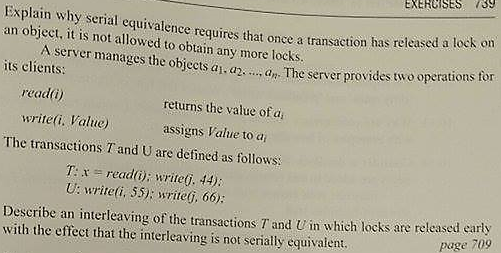
\includegraphics[width = \linewidth]{assignment168}
\end{figure}
The reason why serial equivalence requires that once a transaction has released a lock on an object, it is not allowed to obtain any more locks is the following:\\
If a transaction locks an object after already having released it once, other transactions could potentially try to access and manipulate the object. This could result in the transaction ending up with a wrong result e.g. if a bank transaction is not serial equivalent, there could be to much money or to little in an account after the transaction has ended.\\\\
A non serial equivalent interleaving of the transactions \textit{T} and \textit{U} could be:\\
\textit{U}: write(i,55)
\textit{T}: x = read(i)
\textit{T}: write(j,44)
\textit{U}: write(j,66)
